\documentclass[conference]{IEEEtran}
\IEEEoverridecommandlockouts
% The preceding line is only needed to identify funding in the first footnote. If that is unneeded, please comment it out.
\usepackage{cite}
\usepackage{amsmath,amssymb,amsfonts}
\usepackage{algorithmic}
\usepackage{graphicx}
\usepackage{textcomp}
\usepackage{xcolor}
\usepackage[spanish, mexico]{babel}
\def\BibTeX{{\rm B\kern-.05em{\sc i\kern-.025em b}\kern-.08em
    T\kern-.1667em\lower.7ex\hbox{E}\kern-.125emX}}
\begin{document}

\title{Informe del Proyecto de Complejidad y Optimización\\
}

\author{\IEEEauthorblockN{Juan Felipe Monsalve Vargas}
\IEEEauthorblockA{202160145 \\
juan.felipe.monsalve@correounivalle.edu.co}
\and
\IEEEauthorblockN{Kevin Stiven Gil}
\IEEEauthorblockA{202159863 \\
kevin.gil@correounivalle.edu.co}
\\
\IEEEauthorblockN{Leider Santiago Cortés Hernández}
\IEEEauthorblockA{202159879 \\
cortes.leider@correounivalle.edu.co}
\and
\IEEEauthorblockN{Nicolás Prado León}
\IEEEauthorblockA{202160073 \\
nicolas.prado@correounivalle.edu.co}
}

\maketitle

\section{Introducción}
El problema de encontrar una ubicación óptima para un evento masivo como un concierto puede analizarse desde la perspectiva de la logística y la equidad en el acceso. Este tipo de problemas tiene aplicaciones reales en la planificación urbana y la gestión de servicios públicos. En este proyecto, se modela el departamento del Valle del Cauca como una cuadrícula de N x N km, y se busca hallar un punto que minimice la suma de distancias Manhattan a las ciudades, sin que ese punto coincida con la posición de alguna de ellas, ni beneficie de manera desproporcionada a una ciudad sobre otra.

\section{Objetivos}

\subsection{Objetivo General}

Determinar la ubicación óptima de un concierto dentro del departamento
del Valle del Cauca mediante un modelo de optimización utilizando
distancia Manhattan, garantizando equidad en el acceso desde distintas
ciudades y evitando la localización en zonas que favorezcan a una en
particular.

\subsection{Objetivos Específicos}
\begin{itemize}
	\item
	Modelar matemáticamente el problema como un caso de programación
	entera usando restricciones sobre coordenadas y distancia Manhattan.
	\item
	Diseñar e implementar una interfaz gráfica en Python que permita
	ingresar datos, generar archivos válidos para MiniZinc y ejecutar el
	modelo.
	\item
	Utilizar MiniZinc como herramienta de resolución para obtener la
	ubicación óptima del concierto, aplicando el solver Gecode.
	\item
	Realizar pruebas con diferentes distribuciones de ciudades y tamaños
	del plano, evaluando el comportamiento y desempeño del modelo.
	\item
	Analizar los resultados obtenidos para verificar la equidad y
	eficiencia del modelo frente a escenarios reales y simulados.
\end{itemize}

\section{Modelo del Problema}
Se define un plano de coordenadas enteras donde se ubican M ciudades. Se
usan las siguientes variables:

\begin{itemize}
	\item
	\textbf{\texttt{x\_concierto}, \texttt{y\_concierto}:} coordenadas enteras de la ubicación del
	concierto.
	\item
	\textbf{\texttt{ciudad\_x[i]}, \texttt{ciudad\_y[i]}:} coordenadas de la ciudad \texttt{i}.
	\item
	\textbf{\texttt{dx[i]}, \texttt{dy[i]}:} distancia absoluta en \texttt{x} y \texttt{y} del concierto a la
	ciudad \texttt{i}.
\end{itemize}

\subsection{Restricciones}

\begin{itemize}
	\item
	\texttt{dx[i]} = \textbar \texttt{x\_concierto} - \texttt{ciudad\_x[i]}\textbar
	\item
	\texttt{dy[i]} = \textbar \texttt{y\_concierto} - \texttt{ciudad\_y[i]}\textbar
	\item
	El concierto no puede ubicarse en la posición de ninguna ciudad.
\end{itemize}

\subsection{Función Objetivo}
Minimizar la suma de las distancias Manhattan:
\begin{equation}
	\text{total\_distancia} = \sum_{i=1}^{M} (dx[i] + dy[i])
\end{equation}

\section{Modelo del Problema}

Se modela el problema sobre un plano cartesiano discreto de tamaño $N \times N$, donde $N$ representa el número de filas y columnas. Cada ciudad está localizada mediante coordenadas enteras $(x_i, y_i)$, y se busca ubicar un concierto en una posición $(x_c, y_c)$ tal que se minimice la suma de las distancias Manhattan desde el concierto hacia cada ciudad.

\subsection*{Variables de decisión}

\begin{itemize}
    \item $x_c$, $y_c$: Coordenadas del concierto. Variables de decisión enteras con dominio $[0, N-1]$.
\end{itemize}

Estas variables están sujetas a las condiciones de no negatividad y cota superior de forma implícita por el dominio definido:
\[
x_c, y_c \in \{0, 1, \dots, N-1\}
\]

\subsection*{Parámetros del modelo}

\begin{itemize}
    \item $M$: Número total de ciudades.
    \item $(x_i, y_i)$: Coordenadas fijas de la ciudad $i$, con $i \in \{1, \dots, M\}$.
\end{itemize}

\subsection*{Variables auxiliares}

Para modelar las distancias absolutas, se definen:

\begin{itemize}
    \item $dx_i = |x_c - x_i|$: Distancia en el eje $x$ entre el concierto y la ciudad $i$.
    \item $dy_i = |y_c - y_i|$: Distancia en el eje $y$ entre el concierto y la ciudad $i$.
\end{itemize}

Dado que la mayor distancia entre dos coordenadas en el plano es $|0 - (N - 1)| = N - 1$ en cada eje, la máxima distancia Manhattan entre dos puntos en el plano es:

\[
\max(\text{distancia}) = (N - 1) + (N - 1) = 2N - 2
\]

Por tanto, se define el dominio de las variables auxiliares como:
\[
dx_i, dy_i \in [0, 2N]
\]
lo cual garantiza que el modelo esté acotado correctamente, sin excluir posibles soluciones.

\subsection*{Restricciones}

\begin{itemize}
    \item Modelado de la distancia absoluta en ambos ejes, para cada ciudad $i$:
    \[
    dx_i = |x_c - x_i| \quad \forall i \in \{1, \dots, M\}
    \]
    \[
    dy_i = |y_c - y_i| \quad \forall i \in \{1, \dots, M\}
    \]
    Dado que el uso directo del valor absoluto en funciones objetivo no está permitido en MiniZinc, estas expresiones se modelan con desigualdades equivalentes:
    \[
    dx_i \geq x_c - x_i,\quad dx_i \geq x_i - x_c
    \]
    \[
    dy_i \geq y_c - y_i,\quad dy_i \geq y_i - y_c
    \]

    \item Se evita que el concierto se ubique en la misma posición exacta de una ciudad:
    \[
    (x_c \ne x_i) \lor (y_c \ne y_i) \quad \forall i \in \{1, \dots, M\}
    \]
\end{itemize}

\subsection*{Función Objetivo}

Minimizar la suma total de las distancias Manhattan entre el concierto y las ciudades:

\[
\min \sum_{i=1}^{M} (dx_i + dy_i)
\]

Esta expresión representa la suma de las distancias absolutas en ambos ejes, que corresponde a la distancia Manhattan total desde el punto $(x_c, y_c)$ a todas las ciudades.


\section{Pruebas Realizadas}
Se utilizaron los siguientes conjuntos de datos:

\subsection{Entrada 1}

Con los valores:

\begin{align*}
	N &= 10 \\
	\texttt{num\_ciudades} &= 4 \\
	\texttt{ciudad\_x} &= \{1,\ 3,\ 2,\ 1\} \\
	\texttt{ciudad\_y} &= \{9,\ 9,\ 7,\ 4\}
\end{align*}

\begin{figure}[h]
	\centering
	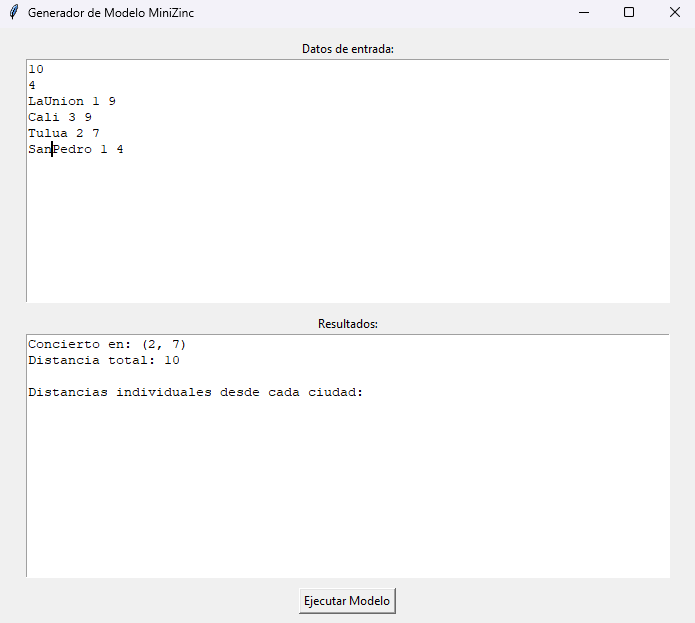
\includegraphics[width=1.0\linewidth]{images/entrada1}
	\caption{Entrada 1.}
	\label{fig:entrada1}
\end{figure}

\subsection{Entrada 2}

Correspondiente al ejemplo del enunciado, cuyos valores son:

\begin{align*}
	N &= 12 \\
	\texttt{num\_ciudades} &= 5 \\
	\texttt{ciudad\_x} &= \{2,\ 10,\ 11,\ 0,\ 1\} \\
	\texttt{ciudad\_y} &= \{3,\ 2,\ 0,\ 3,\ 2\}
\end{align*}

\subsection{Entrada 3}

Con los valores:

\begin{align*}
	N &= 15 \\
	\texttt{num\_ciudades} &= 10 \\
	\texttt{ciudad\_x} &= \{1,\ 3,\ 2,\ 1,\ 4,\ 6,\ 8,\ 10,\ 11,\ 13\} \\
	\texttt{ciudad\_y} &= \{14,\ 13,\ 11,\ 8,\ 5,\ 6,\ 4,\ 3,\ 7,\ 2\}
\end{align*}

\begin{figure}[h]
	\centering
	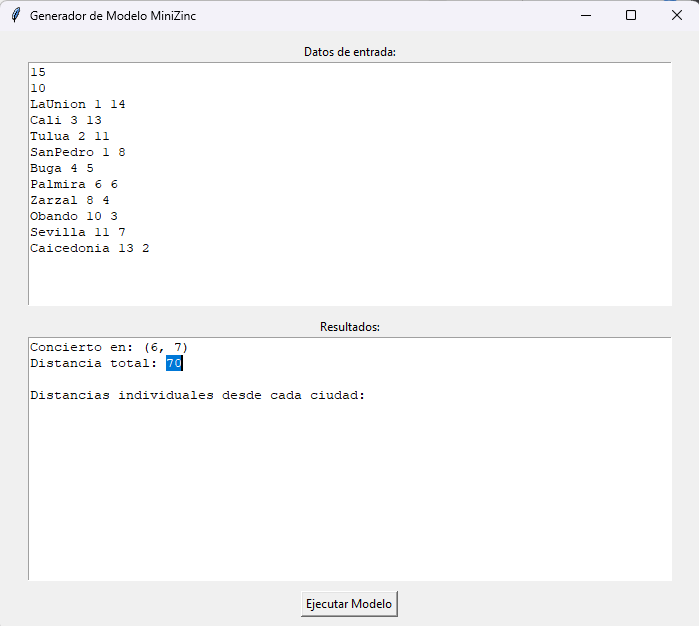
\includegraphics[width=1.0\linewidth]{images/entrada3}
	\caption{Entrada 3.}
	\label{fig:entrada3}
\end{figure}

En todos los casos, se pudo obtener la ubicación óptima del concierto que
minimiza la suma de las distancias a las ciudades.

\section{Análisis de las Pruebas Realizadas}

Al aumentar el valor de N o la cantidad de ciudades, el espacio de
búsqueda se expande, haciendo más compleja la solución. Se observó que:

\begin{itemize}
	\item
	El tiempo de resolución crece moderadamente con más ciudades.
	\item
	Si las ciudades están dispersas uniformemente, el concierto tiende a
	ubicarse en una posición central.
	\item
	Si hay aglomeración de ciudades en un sector, el concierto se desplaza
	hacia ese sector.
\end{itemize}

Se garantiza equidad al evitar que el concierto quede exactamente en una
ciudad, y la función objetivo asegura la minimización del desplazamiento
global.

\section{Conclusiones}
\begin{itemize}
	\item
	El problema fue modelado exitosamente como un caso de programación
	lineal con variables discretas, utilizando la distancia Manhattan como
	métrica clave de optimización.
	\item
	El uso de MiniZinc facilitó la formulación clara y expresiva del
	problema, facilitando la inclusión de restricciones y objetivos sin
	necesidad de codificar algoritmos complejos de búsqueda manual.
	\item
	La interfaz en Python simplifica la recolección de datos y automatiza
	la generación de instancias para MiniZinc.
	\item
	El modelo es flexible: se adapta a distintas configuraciones y tamaños
	de entrada, mostrando que el comportamiento es coherente frente a
	escenarios simples y también más complejos (como el caso con 10
	ciudades).
	\item
	El modelo se comporta de forma robusta frente a distintas
	distribuciones y cantidades de ciudades.
	\item
	Este ejercicio fortalece el entendimiento de modelado matemático y
	optimización aplicada, fundamentales para la ingeniería moderna.
	\item
	El análisis de las pruebas evidenció que el modelo reacciona
	adecuadamente ante ciudades alineadas, dispersas o agrupadas,
	reflejando el desplazamiento necesario en la posición del concierto
	para minimizar la distancia total.
	\item
	En términos generales, el proyecto refleja una comprensión integral de
	la optimización aplicada a problemas reales, con capacidad de
	extenderse fácilmente a variantes del problema, cómo ponderar ciudades
	o añadir restricciones geográficas.
\end{itemize}

\end{document}
